\graphicspath{{Kapitel/Kapitel3_Systembeschreibung/Images/}}

Das Hauptthema mit dem sich diese Arbeit beschäftigt ist das Virtual Reality Programm C.LABEL-VR. Damit dieses Programm entwickelt und betrieben werden kann bedarf es aber einiger erwähnenswerter Komponenten, welche das System um die Applikation herum repräsentieren. Dazu gehört vor allem eine Virtual Reality Brille. Warum hierfür die Oculus Rift genommen wurde und warum Virtual Reality für solch eine Applikation geeigneter ist als vergleichbare Technologien wird in Kapitel \ref{sec:VRBrille} erläutert. Der Computer der für den Betrieb der VR-Brille benutzt wurde und was bei der Auswahl dessen Komponenten wichtig war ist in Kapitel \ref{sec:VR-Rechner} beschrieben. Mit den eben genannten Komponenten lässt sich eine VR-Applikation zwar ausführen, jedoch nicht entwickeln. Dafür ist zusätzlich eine Entwicklungsumgebung notwendig, genauer gesagt eine Spiel-Engine (\textit{Game Engine}). Welche Engine in dieser Arbeit verwendet wurde und welche grundlegenden Konzepte dieser wichtig für die Entwicklung waren, wird in Kapitel \ref{sec:VREngine} beschrieben.

\section{Komponente 1: Die VR-Brille}
\label{sec:VRBrille}

Wie schon erwähnt, war die praktische Hauptaufgabe dieser Arbeit die Realisierung einer Applikation zur Annotation von Punktwolken in einer dreidimensionalen Umgebung. Hierfür wurde die Virtual Reality Technologie verwendet, welche im Kapitel \ref{sec:VirtualReality} näher erläutert wird. Diese ist jedoch nicht die einzige Technologie die für diesen Anwendungsfall in Frage kam. Auch die \textit{Augmented Reality (AR)} bietet einige interessante Konzepte um solch eine Applikation zu entwickeln. Warum hierbei aber VR zu bevorzugen ist, wird im folgenden Abschnitt \ref{sec:WhyVR} erläutert. Im anschließenden Abschnitt \ref{WhyOculus} wird gezeigt welche VR-Brillen für die Entwicklung in Frage kamen und warum die Oculus Rift aus diesen ausgewählt wurde.

\subsection{Warum VR die passende Technologie für C.LABEL-VR ist}
\label{sec:WhyVR}

Um das \glslink{glos:Labeling}{Labeling} von Daten, insbesondere Punktwolken, im dreidimensionalem Raum zu verwirklichen, gibt es zwei wesentliche Technologien die dafür relevant erscheinen. Neben VR, das schon vorgestellt wurde (Kapitel \ref{sec:VirtualReality}), gibt es noch die Augmented Reality Technologie. Unter AR versteht man die direkte oder indirekte Sicht auf die reale, physische Welt, welche durch digitale Inhalte erweitert wird. Dies wird vor allem durch Smartphones oder \acrshort{acr:AR}-Brillen realisiert. Bei einem Smartphone hat man beispielsweise einen indirekten Blick auf die reale Umgebung durch das Display, welches ein Live-Bild oder ein aufgenommenes der Kamera anzeigt. Diesen Bildern können nun digitale Inhalte hinzugefügt werden. Bei einer Brille (vgl. Abbildung \ref{fig:AR-Brillen}) sieht man durch die Gläser direkt auf die physische Welt. Hierbei fungieren die Gläser als Display, welche in der Lage sind holographische Objekte anzuzeigen. Dies führt zu einer, für den Benutzer, sehr immersiven Vermischung der realen und der digitalen Welt. Üblicherweise ist es bei diesen Brillen sogar möglich durch Gesten, die mittels Händen durchgeführt werden, mit den Hologrammen zu interagieren.\\

\begin{figure}%
    \centering
    \subfloat[Microsoft Hololens \acrshort{acr:AR}-Brille]{{\includegraphics[width=5cm]{Hololens}\label{fig:Hololens}}}%
    \qquad
    \subfloat[Meta 2 \acrshort{acr:AR}-Brille]{{\includegraphics[width=4cm]{Meta2}\label{fig:Meta2}}}%
    \caption{Die zwei potentiellen \acrshort{acr:AR}-Brillen}\label{fig:AR-Brillen}%
\end{figure}

\subsubsection{Eignung von \acrlong{acr:AR} für 3D-Annotation}
Der, im Rahmen dieser Arbeit, entwickelte Prototyp zur \glslink{glos:Labeling}{3D-Datenannotation} ist nicht nur als Nutzungssoftware geplant, sondern dient auch als Anschauungsmaterial, beispielsweise für Messen. Zieht man diese Tatsache in Betracht, eignet sich \acrlong{acr:AR} sehr gut für diesen Zweck. Es wirkt durch die Vermischung von realen und digitalen Inhalten nämlich sehr futuristisch. Zudem ist das direkte einblenden holographischer Inhalte, durch eine \acrshort{acr:AR}-Brille, zum Zeitpunkt der Erstellung dieser Arbeit, noch wenig verbreitet (Microsoft Hololens wurde nur wenige Tausend mal verkauft \cite{bib:HololensVerkaufszahlen}), was bei unwissenden Benutzern zu einem beeindruckenden Effekt führt. Des Weiteren bietet die \acrlong{acr:AR} Technologie viele Möglichkeiten, die für zukünftige \glslink{glos:Labeling}{Labeling}-Methoden relevant sein könnten. Den heutigen \acrshort{acr:AR}-Brillen ist es durch \glspl{glos:Tiefenkamera} möglich Objekte und deren Distanzen zur Brille wahrzunehmen. Folglich könnte ein zukünftiger Ansatz sein, eine Punktwolke der Umgebung, wie sie in Abbildung \ref{fig:CloudInClabel} zu sehen ist, mit einer \acrshort{acr:AR}-Brille zu erstellen. Diese kann anschließend vor Ort, in der Umgebung in der die Punktwolke erstellt wurde, klassifiziert werden.\\ %TODO Dieser Ansatz könnte ausführlicher sein. 

Ein wichtiger Punkt der ebenfalls betrachtet werden muss ist die Bedienung der Brille bzw. die Interaktion mit den digital dargestellten Objekten und Informationen. Die Steuerung von \acrshort{acr:AR}-Brillen erfolgt handelsüblich über Gesten, welche mit der Hand bzw. den Händen getätigt werden. Ob diese Art der Interaktion für den hier gewünschten Anwendungsfall passend wäre, lässt sich im Voraus schwer feststellen. Denkbar wäre, dass sich der Benutzer durch intuitive Gesten, die man auch bei realen Objekten nutzt, schnell an die Bedienung des Tools gewöhnen würde. Andererseits könnte die Selektion der Elemente einer Punktwolke zu ungenau sein, da die Brille die Position der Hand nicht richtig interpretiert bzw. diese nicht richtig zur Position der digitalen Inhalte interpretiert. Eine genaue Einschätzung der Bedienung für solch einen Anwendungsfall kann allerdings nur gegeben werden indem man einen \glslink{glos:Labeling}{Labeling}-Prototypen erstellt und ihn anschließend über längere Zeit testet. Dies ist im Zeitrahmen einer Masterarbeit jedoch nicht möglich. Falls sich nämlich die Steuerung als ungeeignet herausstellt bleibt nicht genug Zeit für eine Neuentwicklung auf einer anderen Plattform.\\  

Darüber hinaus gibt es natürlich auch Aspekte die gegen die \acrshort{acr:AR}-Technologie sprechen. Die \glslink{glos:Labeling}{Klassifizierung} einer Punktwolke mit dieser Technik ist an einem normalen Büro-Arbeitsplatz nicht möglich, zumindest nicht in einem Maßstab in dem es sinnvoll wäre. Die holographischen Punkte kollidieren, wenn sie darauf programmiert sind, mit der Umgebung und so würde Darstellung des \glslink{glos:Umfeldmodell}{Umfeldmodells} verfälscht werden. Auch wenn sie das nicht tun, dann wäre die Umgebung selbst immer noch ein Hindernis für den Benutzer, denn man möchte sich ja durch die Punktwolke bewegen. 

Des Weiteren sind bei \acrshort{acr:AR}-Brillen die vorherrschenden Lichtbedingungen ein großer Faktor, welche die Funktionalität gewisser Anwendungsfälle beeinflussen können. Wird beispielsweise eine Lichtquelle zu sehr von einem Objekt reflektiert, kann dieses von der \gls{glos:Tiefenkamera} der Brille nicht mehr richtig erfasst werden. Somit stimmt das \gls{glos:Umfeldmodell} nicht mehr mit der Realität überein. Zudem wird nicht nur die Funktionalität von Lichteinflüssen gestört, sondern auch die Darstellung der Hologramme. Bei zu viel Licht sind diese deutlich schwerer zu erkennen, vergleichbar mit der Nutzung eines Laptops im Freien, bei dem der Bildschirminhalt wegen zu heller Umgebung ebenfalls schlecht erkennbar ist. 

Für die Entwicklung selbst ist es ebenfalls hinderlich das es, zum Zeitpunkt der Erstellung dieser Arbeit, wenig Dokumentationen und Hilfestellungen, zum Beispiel in Entwicklerforen, gibt. Dies ist jedoch üblich für Technologien, die noch nicht lange auf dem Markt sind. Zu guter Letzt ist noch der finanzielle Faktor zu berücksichtigen. Durch die Aktualität der Technologie ist diese auch sehr teuer. Der Preis für eine \acrshort{acr:AR}-Brille kann dabei den Betrag von 5.000 Euro überschreiten \cite{bib:HololensPreis}.   

\subsubsection{Eignung von \acrlong{acr:VR} für 3D-Annotation} 

Die \acrlong{acr:VR} Technologie bietet den großen Vorteil, beliebig große Räume virtuell begehbar zu machen, ohne sich in der realen Welt selbst bewegen zu müssen. Dies ermöglicht die Bewegung durch Punktwolken, die im dreidimensionalen Raum dargestellt sind, an jedem üblichen Arbeitsplatz eines Büros. Des weiteren wirkt die Steuerung der \acrshort{acr:VR}-Brillen mittels den zugehörigen Controllern zum Teil sehr ausgereift. Die Positions- und Bewegungserkennung des Benutzers wird als \textit{\glqq äußerst präzise\grqq} beschrieben \cite{bib:ControllerTest}. Dies ist sehr wichtig um die Handhabung der Anwendung für den späteren Endnutzer so angenehm wie möglich zu machen.

Für die Entwicklung von \acrshort{acr:VR}-Applikationen selbst ist zu sagen, dass es mittlerweile sehr umfassende Dokumentationen, Anleitungen und Beiträge zu den jeweiligen Plattformen und \glspl{acr:SDK} gibt. Dies hängt damit zusammen, dass sich die \acrlong{acr:VR} Technologie schon etwas länger auf dem Markt befindet und die Zahl der Entwickler für \acrshort{acr:VR}-Applikationen stetig steigt. Dies ist vermutlich nicht zuletzt der Tatsache zu verdanken, dass die Preise für \acrshort{acr:VR}-Brillen gesunken sind. Der Preis einer Oculus Rift beträgt zum Zeitpunkt dieser Arbeit 449 Euro. Sowohl die zahlreichen Informationen für Entwickler als auch der niedrige Preis der Hardware sprechen, neben den zuvor genannten Aspekten, für die Wahl von \acrlong{acr:VR} als Plattform für die Entwicklung von 3D-\glslink{glos:Labeling}{Labeling}.\\

Was mit der \acrshort{acr:VR}-Technologie nicht ohne Weiteres funktioniert, ist die physische Begehung einer Punktwolke. Zwar bietet die Technik die Möglichkeit durch zusätzliche Sensoren die Bewegungen des Benutzers in die virtuelle Welt zu übersetzen, jedoch funktioniert dies nur auf begrenztem Raum und ist unmöglich an einem üblichen Büro-Arbeitsplatz durchführbar. Der reale begehbare Raum muss nämlich durch diese Sensoren abgesteckt werden und ist somit durch deren Reichweite und Genauigkeit begrenzt. Ein weiter Negativaspekt ist, dass viele Benutzer von \acrshort{acr:VR}-Brillen über Übelkeit klagen. In manchen Tests sind es mehr als 50 Prozent aller Teilnehmer, vor allem wenn es sich um Frauen handelt \cite{bib:VRSickness}. 

\subsubsection{Entscheidung}
Für die Wahl des passenden Mediums, auf dem das dreidimensionale \glslink{glos:Labeling}{Labeling} entwickelt werden soll, sind mehrere Faktoren entscheidend. Diese Faktoren ergeben sich danach, wie sehr sich etwas für die genannte Anwendung eignet. Zunächst ist es wichtig eine Punktwolke deutlich und nach Möglichkeit im richtigen Maßstab darzustellen. Hier kommt die \acrlong{acr:AR}-Technologie sicherlich an ihre Grenzen. Grund dafür ist die ungenaue Interaktion mit der Umgebung und die lichtempfindlichen Darstellung digitaler Inhalte. In der virtuellen Realität dagegen kann eine solche Wolke problemlos bei jeder Bedingung angezeigt werden, da die reale Umgebung nicht berücksichtigt wird. Sogar der Maßstab kann gut eingehalten werden, da dem virtuellen Raum keine Grenzen gesetzt sind, sodass beliebig große Umfeldmodelle an jedem Arbeitsplatz dargestellt werden können.\\

Auch die Steuerung spricht für den Einsatz von \acrlong{acr:VR}. Zwar ist das Konzept der Greif-Steuerung der Meta 2 ein guter Ansatz, da diese aber noch nicht zuverlässig und genau funktioniert, ist sie für die Selektion vieler Objekte nicht gut geeignet. Dagegen bietet die Steuerung durch Controller bei \acrshort{acr:VR}-Brillen deutlich mehr Möglichkeiten eine gute Bedienung für die gewünschte Anwendung zu entwickeln. Die Tasten eines solchen Controllers können vom Entwickler nämlich nach Wunsch programmiert werden wogegen die Gesten für \acrshort{acr:AR}-Brillen nicht verändert bzw. nicht neu erstellt werden sollten \cite{bib:NewGesture}. Zudem gibt es, durch die deutlich frühere Markteinführung, viel mehr Dokumentationen und Hilfestellungen im Bereich \acrlong{acr:VR}, was die Entwicklung deutlich erleichtert.
Aufgrund der eben genannten Vorteile von \acrshort{acr:VR} gegenüber \acrshort{acr:AR} wird für die Entwicklung, im Rahmen dieser Arbeit, \textbf{\acrlong{acr:VR}} verwendet.\\

\subsection{Warum die Oculus Rift verwendet wurde}
\label{WhyOculus}

Die, in dieser Arbeit, entwickelte Methode zur \glslink{glos:Labeling}{3D-Datennotation} ist vorwiegend für einen normalen Arbeitsplatz im Büro konzipiert, also einen Platz an dem man einen Desktop-Computer zur Verfügung hat. Deswegen macht es keinen Sinn \acrshort{acr:VR}-Brillen in Betracht zu ziehen die von einem mobilen Gerät betrieben werden (\textit{Samsung Gear VR}), da diese deutlich weniger Leistung und eine schlechtere Bedienung haben als Geräte für einen Desktop-PC. Auch die Nutzung der \textit{Playstation VR} ist nicht sinnvoll, da zum Betrieb eine Playstation 4 nötig ist, welche in den wenigsten Unternehmen vorhanden sein dürfte.

Für das \glslink{glos:Labeling}{Klassifizieren} im dreidimensionalen Raum ist eine gute Darstellung und Bedienung notwendig. Bei \acrshort{acr:VR}-Brillen, die einen Desktop-PC als Recheneinheit haben wird beides geboten. Durch die hohe Leistung eines performanten Computers kann der dreidimensionale Raum hochauflösend dargestellt werden. Auch die genaue, für Spiele konzipierte, Steuerung über Controller kommt einem \glslink{glos:Labeling}{Labeling}-Tool zugute. Zum Zeitpunkt der Erstellung dieser Arbeit, gibt es zwei relevante VR-Brillen aus dieser Sparte, die \textit{Oculus Rift} und die \textit{HTC Vive}.

\begin{figure}%
    \centering
    \subfloat[HTC Vive \acrshort{acr:VR}-Brille mit Controllern \cite{bib:VivePic}]{{\includegraphics[width=5cm]{Vive}\label{fig:Vive}}}%
    \qquad
    \subfloat[Oculus Rift \acrshort{acr:VR}-Brille mit Controllern \cite{bib:OculusPic}]{{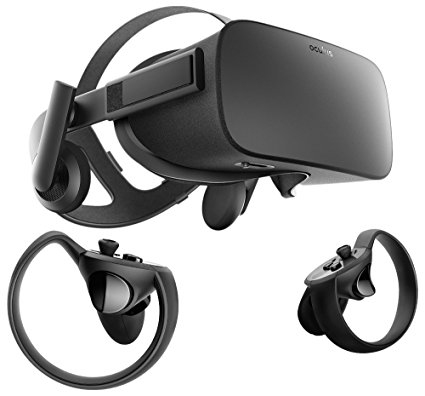
\includegraphics[width=3cm]{Oculus}\label{fig:Oculus}}}%
    \caption{Die zwei potentiellen \acrshort{acr:VR}-Brillen}\label{fig:VR-Brillen}%
\end{figure}

\subsubsection{Oculus Rift}
Mit 470 Gramm ist die Oculus Rift (vgl. Abbildung \ref{fig:Oculus}) deutlich leichter als andere Modelle, wie beispielsweise die HTC Vive mit 600 Gramm oder die Playstation VR mit 610 Gramm \cite{bib:OculusTestTragekomfort}. Dies ist für längeres Arbeiten mit ihr sehr vorteilhaft, da schwere Brillen oft schon nach kurzer Zeit störend beim Tragen sind. Des weiteren lässt sich die Brille problemlos an jedem handelsüblichen Büro-Arbeitsplatz verwenden. \textit{\glqq Oculus empfiehlt, die Kameras im Abstand von zwei Metern nebeneinander zu platzieren – bei einem klassischen PC-Arbeitsplatz also links und rechts neben dem Monitor. Das funktioniert in der Praxis gut, man kann sich mit diesem Aufbau ungefähr jeweils einen Schritt in alle Richtungen bewegen\grqq} \cite{bib:OculusTouchTest}. Auch in Sachen Steuerung ist die Oculus Rift anderen Modellen überlegen. Durch die sogenannten \textit{Oculus Touch} Controller, mit denen man virtuell nicht nur Greifen, sondern auch Daumen und Zeigefinger bewegen kann, gelingen ihr \textit{\glqq deutlich feinere Bewegungen\grqq} als beispielsweise der HTC Vive \cite{bib:OculusTouchTest}. Dies bietet für die Entwicklung einer Lösung zur Markierung vieler Objekte zahlreiche Möglichkeiten.\\

Was bei der Oculus Rift nicht so gut funktioniert, wie bei anderen Brillen ist das \gls{glos:Roomscaling}, also das Erfassen der Bewegungen des Benutzers durch einen größeren Raum. Dieser Aspekt erschwert somit das räumliche begehen einer Punktwolke. Für dieses Verfahren gibt es bei der Rift zwei Methoden. Einmal mit zwei Kameras (kleine Überwachungsfläche), die sich im Abstand von drei Metern in zwei Raumecken gegenüberstehen und eine mit drei Kameras (größere Überwachungsfläche). Beide Methoden funktionieren nicht einwandfrei und auch nicht so gut wie bei der HTC Vive \cite{bib:OculusTouchTest}.

\subsubsection{HTC Vive}
Die HTC Vive (vgl. Abbildung \ref{fig:Vive}) punktet mit dem ausgeklügelten Lighthouse Tracking System, welches in Zusammenarbeit mit VALVE entwickelt wurde \cite{bib:Lighthouse}. Das System kann die Kopfbewegungen des Benutzers durch mehr als 70 Sensoren auf bis zu ein zehntel eines Grades messen \cite{bib:ViveTest}. Die Sensoren sind dabei sowohl in die Brille integriert als auch extra positioniert. Auch die Controller werden durch dieses System erfasst, was zu einer genauen Übertragung der physischen Handbewegungen in die virtuelle Welt führt. Dies kommt der Auswahl zahlreicher Objekte, wie es bei der Klassifizierung von Punkten notwendig ist, sehr entgegen. Auch eine gute Darstellung ist aufgrund zweier Displays gewährleistet, die jeweils eine Auflösung von 1080 auf 1200 Pixel haben. Bei diesen Displays kommt es weder zu Verzerrungen des Bildes (\textit{\glqq lens distortion\grqq} \cite{bib:ViveTest}) noch zu Pixelfehlern. Ebenfalls nützlich, vor allem am Arbeitsplatz, ist die Bluetooth-Funktion der Vive. Damit ist es möglich sein Smartphone mit der Brille zu verbinden und somit eingehende Emails oder Ähnliches zu lesen und zu beantworten, ohne die Brille absetzen zu müssen.\\  

Der große Unterschied zwischen Vive und Rift liegt bei der Bedienung durch die unterschiedlichen Controller. Hier hat die HTC-Brille das Nachsehen, weil sie durch Anatomie der Controller weniger Möglichkeiten zur Interaktion in der virtuellen Umgebung bietet. Die sogenannten \textit{Wands} bieten nämlich keinerlei Funktionen die es ermöglichen eine Hand nachzuahmen, um beispielsweise einzelne Finger zu bewegen und somit virtuelle Objekte greifen zu können. Im Hinblick auf eine durchdachte Steuerung für die Auswahl und Markierung vieler Punkte in einer Punktwolke gibt es somit weniger Möglichkeiten diese zu entwickeln.

\subsubsection{Entscheidung}
Bleibt noch die Frage zu klären welche Brille verwendet werden soll. Diese Frage ist schwerer zu beantworten als die vorherige. Die zwei potentiellen \acrshort{acr:VR}-Brillen, also Oculus Rift und HTC Vive, sind beide geeignete Kandidaten. Die Vive punktet durch gutes \gls{glos:Roomscaling} und gutes Erfassen der Brille und der Controller, wogegen die Oculus Rift guten Tragekomfort und gut durchdachte Controller-Bedienung bietet. 

Wichtig für die Entwicklung einer \glslink{glos:Labeling}{3D-Datennotation} ist aber nicht, ob man sich physisch, also mittels \gls{glos:Roomscaling} durch die Punktwolke bewegen kann, sondern wie man die klassifizierbaren Punkte markieren bzw. auswählen kann. Da hierfür die Oculus Touch Controller mehr Möglichkeiten bieten wird für die Entwicklung eines \acrshort{acr:VR}-\glslink{glos:Labeling}{Labeling}-Tools die \textbf{Oculus Rift} verwendet. 

\section{Komponente 2: Der Rechner}
\label{sec:VR-Rechner}
Für die Berechnungen, die notwendig sind um Inhalte in der Oculus Rift anzuzeigen, ist nicht die Brille selbst verantwortlich. Diese Aufgabe übernimmt ein separater Computer. Die Brille fungiert dementsprechend nur als Anzeigegerät. Auch die Sensoren sind an den PC angeschlossen um das Erfassen der Brille und der Controller zu gewährleisten. Vor allem die Grafikberechnungen sind sehr aufwendig sind, da die Darstellung von VR-Inhalten zwei mal berechnet werden (für jedes Auge extra) und nicht nur einmal, wie es an einem Bildschirm der Fall ist. Deshalb kann nicht jeder handelsübliche PC oder Laptop dazu verwendet werden eine solche \acrshort{acr:VR}-Brille zu betreiben. Was ein passender Computer für die Nutzung von Virtual Reality bieten muss wird im Folgenden erläutert.\\ 

Wichtig sind zunächst die Basiskomponenten wie ein schneller Prozessor und eine leistungsstarke Grafikkarte. Aber auch ein schneller Arbeitsspeicher mit ausreichender Kapazität ist wichtig damit notwendige Daten so schnell wie möglich zur Verfügung stehen. Für die Wahl, welche Komponenten eingesetzt werden sollen, kann sich an den empfohlenen Spezifikationen des Herstellers orientiert werden (Oculus Rift Recommended System Specs \cite{bib:OculusSpecs}). Diese sind jedoch vorwiegend für den Endnutzer gedacht, bei dem es wichtig ist ein einzelnes Programm für die Brille auszuführen. Für die Entwicklung ist dagegen mehr Leistung notwendig. Soll zum Beispiel eine erstellte Applikation getestet werden, muss nicht nur die Applikation selber ausgeführt werden, sondern auch die Entwicklungsumgebung und zusätzliche \glslink{glos:Debugger}{Fehlerbehebungs-} und  Analyse-Anwendungen. An dieser Stelle darf also nicht gespart werden.\\

Sind die Basiskomponenten ausgewählt, sollte noch geprüft werden ob noch weiteres Zubehör wichtig ist um diese zu betreiben. Da gerade Prozessoren mit hoher \gls{glos:Taktrate} viel Wärme produzieren, muss stets für ausreichende Kühlung gesorgt werden. Bei der Rechner-Konfiguration für diese Masterarbeit wurden beispielsweise, neben einem hochwertigen Prozessorkühler, noch zwei weitere Gehäuselüfter verbaut, um die Abwärme aus dem inneren des Computers heraus zu leiten. 

Zu guter Letzt ist es wichtig ein passendes Mainboard auszuwählen, auf dem alle Komponenten verbaut werden. Für die Oculus Rift werden vier USB-Anschlüsse empfohlen, welche das Mainboard haben muss \cite{bib:OculusSpecs}. Ebenfalls muss das Board genug Platz bieten um die gewählten Komponenten zusammen anbringen zu können. Leistungsstarke Grafikkarten und Prozessorlüfter können zum Teil sehr groß ausfallen. Auch für weitere Aufrüstungen sollte das Board genügend Platz bieten, falls es, zu einem späteren Zeitpunkt, notwendig wäre zusätzliche Komponenten (zweite Grafikkarte) hinzuzufügen. Unter Berücksichtigung der eben genannten Aspekte wurde folgende Rechner-Konfiguration für die Entwicklung verwendet:\\  

\begin{table}[h]
 \begin{tabular}{ll}
  \textbf{Bezeichnung der Komponente} & \textbf{Verwendete Komponente}\\
  \\
  
  \textit{Prozessor:} & Intel® Core™ i7-7700K\\
  \textit{Grafikkarte:} & Gainward GeForce GTX 1070 Phoenix\\
  \textit{Mainboard:} & ASUS PRIME Z270-A\\
  \textit{Arbeitsspeicher(RAM):} & HyperX DIMM 16 GB DDR4-2400 Kit\\
  \textit{Festplatte:} & Samsung 850 Pro 2,5"\ 512 GB\\
  \textit{Netzteil:} & Cooler Master G550M 550W\\
  \textit{Prozessorlüfter:} & Noctua NH-D9L\\
  \textit{Gehäuselüfter:} & 2x Coolink SWiF2-1200 120x120x25\\
  \textit{Gehäuse:} & Cooler Master N300\\
\\
 \end{tabular}
 \caption{Rechner-Konfiguration für die Entwicklungen dieser Arbeit}
 \label{tab:Rechnerkonfig}
 \end{table}


\section{Komponente 3: Die Entwicklungsplattform}
\label{sec:VREngine}

Für die Entwicklung von Virtual Reality Anwendungen werden in der Regel sogenannte Spiel-Engines (\textit{Game Engines}) verwendet. Dies sind komplexe Mehrzweckwerkzeuge für die Erstellung von Multimedia-Inhalten und Videospielen. Eine Spiel-Engine bietet Funktionen, welche die wichtigsten Bereiche der Spielentwicklung abdecken. Eine davon ist die Bildsynthese aus Rohdaten, welche meist geometrische Beschreibungen im zwei- oder dreidimensionalen Raum sind. Die Bildsynthese ist in der Fachsprache besser bekannt als \textit{Rendering}. Der Prozess des Renderings berechnet für jedes angezeigte Bild die Objekte, welche vom Benutzer aus sichtbar sind, deren Oberflächen anhand von ihren Materialeigenschaften und die Lichtverhältnisse des Bildes, die sich unter anderem durch die indirekte Beleuchtung zwischen Körpern äußert. Weitere Funktionen, welche diese Plattformen zu Verfügung stellen, sind beispielsweise Physikalisch Berechnungen (z.B. Schwerkraft), Animationen von Objekten und künstliche Intelligenzfunktionen.\\

Für die Entwicklung von VR-Inhalten ändert sich an den Funktionen, welche die Engine bieten muss nicht all zu viel, da die meisten Anwendungen schon dreidimensional sind. Die meisten Elemente der Bildsynthese müssen allerdings, wie schon im vorherigen Abschnitt \ref{sec:VR-Rechner} erwähnt, zweimal berechnet werden, nämlich für jedes Auge einzeln. Im Folgenden soll erläutert werden warum für diese Arbeit die Unity Engine als Entwicklungsplattform ausgewählt wurde. Anschließend wird diese kurz vorgestellt.  

\subsubsection{Vergleich zwischen Unreal und Unity}

Für die Erstellung von \acrlong{acr:VR} Software gibt es zwei relevante Entwicklungsumgebungen, die gut für das Entwickeln von \acrlong{acr:VR} geeignet sind. Der Grund dafür ist, dass sie schon seit längerem die Erstellung von \acrshort{acr:VR}-Anwendungen unterstützen und dies auf umfassende Weise. Die zwei Entwicklungsumgebungen sind \textit{Unreal Engine 4} und \textit{Unity Engine}. Beide sind für nicht kommerzielle Zwecke zunächst kostenlos benutzbar. Beide Plattformen bieten alles nötige um \acrshort{acr:VR}-Applikationen zu entwickeln, weshalb die Wahl zwischen ihnen eher subjektiv, aufgrund der eigenen Bedürfnisse und Erfahrungen, zu fällen ist.\\ 

In \cite{bib:UEvsUE4} wurden diese beiden Entwicklungsplattformen gegenübergestellt. Im Allgemeinen kann man sagen, dass die Unreal Engine mehr Möglichkeiten für professionelle Spieleentwicklung bietet, da viel Wert auf visuelle Qualität gelegt wird. Beispielsweise wird durch integrierte \gls{glos:PostPr}-Techniken und gute \gls{glos:Shader} das erzeugte Bild besser dargestellt als in Unity. Sie bietet neben dem \gls{glos:Scripting} auch die Gelegenheit, durch C++ Programmierung Module der Engine zu verändern bzw. neue hinzuzufügen. Das gestalten von \glspl{glos:UI} ist mit dem \textit{UMG UI Designer} ebenfalls gut gelöst .\\

Die Unity Engine bietet vor allem Anfängern einen leichten Einstieg in die Welt der Grafik- und Spieleprogrammierung. Im Editor können ganz einfach sogenannte \textit{Game Objects} erstellt werden, denen dann Funktionalitäten und Eigenschaften angehängt werden können. Dies geschieht meist in Form von Skripten, welche oft schon vorgefertigt zur Verfügung stehen. Wenn dies nicht der Fall ist können diese angepasst oder neu erstellt werden. Die große Community der Unity Engine ist hierbei eine große Hilfe.

\subsubsection{Entscheidung}
\label{sec:UnityDecision}
Ein Vorteil den die Unity Engine, im Falle dieser Arbeit, bietet ist Nutzung von C\# als Skript-Sprache. Da  
C.LABEL (vgl. \ref{sec:C.LABEL}) ebenfalls in C\# programmiert wurde können Komponenten, wie etwa das Einlesen von Daten, leicht in die VR-Anwendung übernommen werden. Des Weiteren habe ich selbst, im Rahmen eines Universitätsprojekts, mit dieser Plattform gearbeitet. Ein längeres einarbeiten in die Entwicklungsumgebung wäre demnach nicht nötig. Die Vorteile der Unreal Engine sind, wie schon erwähnt, die visuelle Präsentation und die dabei gebotene Performance. Diese sind vor allem für das Erstellen aufwändiger Landschaften und deren Inhalten von Vorteil. \\

Für die Entwicklung der angestrebten Anwendung spielen jedoch Dinge wie Objekt- und Landschaftsdarstellung keine große Rolle. Viel wichtiger ist sowohl die Möglichkeit der Kompatibilität zur C.LABEL-Anwendung, als auch die vorhandene Entwicklungserfahrung mit einer Plattform. Gerade letzteres ist auf Grund des begrenzten Zeitrahmens einer Masterarbeit von Vorteil, da ohne große Einarbeitung mehr Zeit zum Entwickeln von Funktionalität und Optimierungen bleibt. Aus diesen Gründen wird im weiteren Verlauf dieser Arbeit die \textbf{Unity Engine} als Entwicklungsumgebung verwendet.

\subsubsection{Entwickeln mit Unity}

Die Unity Engine ist eine der am häufigst benutzten Spiel-Engines auf dem Markt. Gerade im Bereich der mobilen Geräte wurden 34 Prozent der 1000 beliebtesten Spiele mit Unity erstellt \cite{bib:Unity34Percent}. Sie ist ebenfalls bei bei Neueinsteigern und Hobbyprogrammierern beliebt, da sie über umfangreiche Lernmaterialien und eine große Entwicklergemeinschaft verfügt. Die Unity Engine unterstützt sowohl alle gängigen großen Plattformen wie PC, Playstation und XBOX, als auch die kleinen mobilen Geräte wie Android, iOS, Nintendo 3DS und PS Vita. Darüber hinaus kann man mit ihr auch Anwendungen für, in der Applikationsentwicklung, weniger gebräuchliche Plattformen wie Samsung SMART TV, oder tvOS erstellen. Wichtig für diese Arbeit ist die umfangreiche Unterstützung von Virtual Reality Brillen, speziell der Oculus Rift. Um die Vorgänge von C.LABEL-VR, die in Kapitel \ref{sec:C.LABEL-VR} beschrieben werden, besser zu verstehen, werden im Folgenden die Grundlagen für die Entwicklung mit Unity etwas näher erläutert.\\ 

Bei der Entwicklung mit Unity werden Anwendungen mittels Szenen konzipiert. Eine Anwendung besteht aus mindestens einer Szene, in der Regel sind es aber mehrere. Jede Szene kann dabei eigene Objekte und Logiken beinhalten und es kann je nach Programmierung des Entwicklers zwischen den Szenen gewechselt werden. Ein klassischer Fall dafür wäre eine Applikation mit einer Hauptmenü- und einer Anwendungsszene. Als erstes wird die Hauptmenü-Szene gestartet und von dieser aus dann, beispielsweise durch die Betätigung eines Knopfes, die Anwendungsszene. In größeren Spielen ist es üblich jeden abgetrennten Bereich im Spiel mit einer extra Szene zu erstellen. Dies dient der Übersicht und der Wartbarkeit, die in Szenen mit zu vielen Objekten nicht mehr gegeben wäre.\\

\begin{figure}%
	\centering
    \includegraphics[width=16cm]{UnityEditor2Circle}
    \caption{Unity Editor, der C.LABEL-VR im Play Mode ausführt.}
    \label{fig:UnityEditor}
\end{figure}

Die Konzeption der einzelnen Szenen geschieht, wie in der Regel in bei jeder Spiel-Engine, über einen Editor (siehe Abbildung \ref{fig:UnityEditor}). 
Die Konzeption beinhaltet beispielsweise die Erstellung von Landschaften und deren Objekten, Anordnung der Objekte und das Testen der Szenen. Für die Erstellung von komplexen 3D-Objekten werden externe Programme wie \textit{Blender} verwendet, deren  Erzeugnisse dann in den Unity Editor importiert werden können \cite{bib:Blender}. Die Erstellung von simplen primitiven Objekten wie Kugeln oder Würfel ist aber auch direkt im Unity Editor möglich.

Mit der Anordnung der Objekte ist zum einen die Platzierung der Objekte innerhalb der Szene gemeint, welche beim Beginn der Szene die Startposition der Objekte ist. Diese kann aber während des Ablaufs der Szene durch Programmierung geändert werden. Zum anderen ist die Anordnung der Objekte innerhalb von Hierarchien gemeint. Dabei werden \textit{Eltern-Kind}-Beziehungen zwischen den Objekten festgelegt, was zur Folge hat, dass Änderungen bei den Eltern sich auch auf die Kinder auswirken. Erstellt man zum Beispiel ein leeres Objekt \glqq Mensch\grqq und ordnet diesem Kopf, Arme, Beine und Oberkörper zu, so kann man das Objekt \glqq Mensch\grqq bewegen und alle Körperteile bewegen sich mit. 

Das Testen einer oder mehrerer Szenen ist mit dem \textit{Unity Play Mode} möglich. Startet man diesen Modus wird die aktuelle Szene, die im Editor geöffnet ist, gestartet ohne die gesamte Applikation vorher kompilieren zu müssen. Das spart dem Entwickler Zeit da zum einen die Kompilierzeit wegfällt und zum anderen die Applikation nicht immer von der Startszene aus gestartet werden muss. Der Editor in der Abbildung \ref{fig:UnityEditor} befindet sich im Play Modus. In diesem Editor sind zwei große Fenster abgebildet, in denen die laufende Szene zu sehen sind. Das obere Fenster zeigt die Editor-Sicht. Innerhalb dieser können Objekte während des Ablaufs der Szene ausgewählt und geändert werden. Im roten Kreis sind markierte Objekte zu sehen, die nach links verschoben wurden. Im unteren Fenster ist die Benutzer-Sicht zu sehen, welche die Szene aus der Sicht des Benutzers zeigt. Dadurch kann überprüft werden wie sich die getätigten Änderungen aus der Editor-Sicht auf die Tatsächliche Sicht des Benutzers auswirken. Auch hier sieht man im roten Kreis die Objekte die im Editor verschoben wurden.\\

Die erwähnten Objekte, welche sich in den einzelnen Szenen befinden, werden in Unity \textit{Gameobjects} genannt. Ein Gameobject ist die übergeordnete Klasse für alle Arten von Objekten in Unity, beispielsweise 2D- und 3D-Objekte, aber auch Elemente von Benutzeroberflächen. Jedes Objekt in Unity ist also ein Gameobject und es ist möglich diesen Objekten bestimmte Komponenten zuzuordnen. Mit diesen Komponenten lassen sich Eigenschaften und Verhaltensweisen der Objekte festlegen. Jedes Gameobject in Unity hat standardmäßig eine, nicht entfernbare, Komponente die sich \textit{Transform} nennt. Diese legt die Position, Orientierung und Größe des Objekts in der Szene fest. Sichtbare Objekte müssen beispielsweise eine \textit{Mesh Renderer}-Komponente haben, welche die Materialeigenschaften des Objektes festlegt und somit der Unity Engine signalisiert, dass das Objekt bei der Bildsynthese berücksichtigt werden muss. Es kann aber auch unsichtbare Objekte geben, die lediglich eine Logik-Komponente haben, welche beispielsweise Aktionen anderer Objekte überwacht.\\

Die Komponenten legen die Eigenschaften und Verhaltensweisen von Objekten mit Hilfe eines Skriptes fest, welches mit einer bestimmten Programmiersprache erstellt wird. In Unity stehen die Sprachen C\# und JavaScript zur Verfügung. Das Implementieren dieser Skripte wird in der Fachsprache als \textit{Scripting} bezeichnet. Dadurch kann der Programmierer, wie schon erwähnt, die Eigenschaften und das Verhalten von Objekten festlegen und beeinflussen. Zur Veranschaulichung dieses Vorgangs dient die Auflistung \ref{lst:GameObject}. Darin ist ein minimalistischer Grundaufbau eines Skriptes zu sehen, dass ein Objekt unter einer Bedingung größer werden lässt.\\

\begin{lstlisting}[caption={Grundaufbei eines Gameobjects in Unity}, captionpos=t, label=lst:GameObject]
using UnityEngine;

public class TestObject : MonoBehaviour
{
    public static TestObject Instance { get; set; }
    public bool EnableGrowing { get; set; }

    private void Awake()
    {
        Instance = this;
    }
    private void Start()
    {
        Instance.EnableGrowing = true;
    }
    private void Update()
    {
    	if(Instance.EnableGrowing)
        	Instance.transform.localScale += new Vector3(1, 1, 1);
    }
}
\end{lstlisting}
\quad


Ein Skript besteht in der Regel aus einer Klasse, wie beispielsweise \textit{TestObject} in Auflistung \ref{lst:GameObject}, die von der Unity-Basisklasse \textit{MonoBehaviour} erbt. Diese Vererbung führt dazu, dass der Klasse TestObject diverse Funktionen zugeordnet werden, die von der Unity Engine zu gewissen Zeitpunkten aufgerufen werden. Dadurch kann das Verhalten des Objekt gezielt gesteuert werden. Diese Funktionen werden jedoch nur aufgerufen, wenn sie innerhalb der erbenden Klasse auch implementiert werden. All diese Funktionen sind in der Dokumentation der Unity Engine aufgelistet und beschrieben \cite{bib:MonoBehaviour}. Die Klasse TestObject implementiert drei von diesen Funktionen, nämlich \textit{Awake()}, \textit{Start()} und \textit{Update()}.\\

Awake wird als erstes aufgerufen, sobald alle Objekte in Unity geldaen sind und kann somit zur Initialisierung von Referenzen verwendet werden bevor die Szene startet. Im Beispiel wird der statischen Instanz von TestObject die Referenz des geladenen Skripts TestObject zugewiesen. Dieses Vorgehen nennt sich \textit{Singleton-Pattern} und ist eine übliche Methode zum verwalten von Referenzen in Unity \cite{bib:Singleton}. Dadurch ist es für andere Skripte möglich, ohne Instanziierung der Klasse, auf diese zuzugreifen.

Die Methode Start wird vor dem ersten Aufruf von Update ausgeführt, also kurz vor dem Start der Szene. Hier können somit noch Werte zugewiesen werden. \textit{EnableGrowing} wird im Skript TestObject auf den boolschen Wert \glqq wahr\grqq{} gesetzt. Dieser kann dann von anderen Skripten durch das eben beschriebene Singleton-Pattern geändert werden (\textit{TestObject.Instance.EnableGrowing = false}).  

Die Update-Methode ist eine Art Endlosschleife die von der Unity Engine immer wieder aufgerufen wird solange das Skript in einem aktiven Zustand ist. Sie repräsentiert die, in der Fachsprache oft genannte, \textit{Game-Loop}. Alle Vorgänge die während der Laufzeit der Applikation ablaufen sollen müssen also in dieser Funktion implementiert werden. Im Beispiel wird die Größe des Objektes erhöht, solange die Variable EnableGrowing den boolschen Wert \glqq wahr\grqq{} hat. Es gibt darüber hinaus noch einige weitere dieser Methoden innerhalb der MonoBehaviour-Klasse, beispielsweise die Methode \textit{OnEnable()}, die aufgerufen wird wenn das Skript vom inaktiven in den aktiven Zustand wechselt. Mit Hilfe all dieser MonoBehavior-Funktionen lassen sich also Objekte und deren Verhalten manipulieren. Auf diese Weise werden gewünschte Vorgänge in Unity implementiert.\\

In diesem Abschnitt wurden nun grundlegende Vorgänge beschrieben, die wichtig sind um Anwendungen mit Unity zu erstellen. Darunter waren zum Beispiel das Konzipieren von Szenen im Editor und das Scripting, also das Programmieren von Logik für die Anwendung. Damit soll ein Einblick in den Prozess der Entwicklung von C.LABEL-VR gegeben werden. Die Beschreibung der Funktionen von C.LABEL-VR selbst und deren Konzepte sind im folgenden Kapitel \ref{sec:C.LABEL-VR} beschrieben. 






%\subsection{\acrshort{acr:AR}-Brillen im Vergleich}
%\label{sec:ARVergleich}
%Zum Zeitpunkt der Recherche über eine passende \acrshort{acr:AR}-Brille, gibt es zwei potentielle Geräte die in Frage kommen. Diese sind \textit{Microsofts Hololens} und die \textit{Meta 2}. Andere Brillen werden, aufgrund der im voraus erkennbaren Hindernisse, nicht berücksichtigt, wie beispielsweise die \textit{Google Glass}, die ein viel zu kleines Display hat. Wiederum andere sind zu diesem Zeitpunkt noch nicht auf dem Markt wie das \textit{Project Aurora}, welches ebenfalls von Google ist, oder die Brille \textit{castAR}. Im Folgenden werden die zwei potentiellen Brillen, im Hinblick auf die Nutzung für \glslink{glos:Labeling}{3D-Labeling}, näher analysiert.
%
%\begin{figure}%
%    \centering
%    \subfloat[Microsoft Hololens \acrshort{acr:AR}-Brille]{{\includegraphics[width=5cm]{Hololens}\label{fig:Hololens}}}%
%    \qquad
%    \subfloat[Meta 2 \acrshort{acr:AR}-Brille]{{\includegraphics[width=4cm]{Meta2}\label{fig:Meta2}}}%
%    \caption{Die zwei potentiellen \acrshort{acr:AR}-Brillen}\label{fig:AR-Brillen}%
%\end{figure}
%
%\subsubsection{Microsoft Hololens}
%Die Hololens-Brille von Microsoft (vgl. Abbildung \ref{fig:Hololens}) punktet vorwiegend in Sachen Darstellung und räumlicher Interaktion, was aus eigener Erfahrung bekannt ist. Eingeblendete Hologramme wirken auf dieser Brille sehr stabil. Ein Ruckeln oder Nachpositionieren der digital dargestellten Inhalte wurde nie bemerkt. Ebenfalls gut funktioniert die Vermessung des Raums durch die Kameras der Brille. Hologramme interagieren dadurch sehr gut mit der physischen Umgebung, indem sie beispielsweise wie ein realer Gegenstand auf einem Tisch positioniert oder an die Wand gehängt werden können (siehe Abbildung \ref{fig:AR-ObjectPlacement}). Lediglich schlecht ausgeleuchtete Bereiche eines Raumes machen dieser Funktion Probleme. Unter schlechten Lichtverhältnissen entdeckt die Brille beispielsweise eine Wand oder ein Hindernis wo keines ist. Die positiven Merkmale der Hololens sind also eine stabile Darstellung von Hologrammen und eine gute Einbettung dieser in eine physische Umgebung. Im Hinblick auf eine Punktwolke als Hologramm sind diese Merkmale wichtig um die Wolke zuverlässig klassifizieren zu können und somit eine gute Methode für \glslink{glos:Labeling}{3D-Datennotation} zu entwickeln.\\
%
%\begin{figure}%
%    \centering
%    \includegraphics[width=8cm]{HololensObjectPlacement}
%    \caption{Platzierung eines digitalen Objekts auf einem physischen Objekt mit der Microsoft Hololens}
%    \label{fig:AR-ObjectPlacement}%
%\end{figure}
%
%Die Gestensteuerung der Hololens wäre für den Prozess der \glslink{glos:Labeling}{Klassifizierung} von dreidimensionalen Punktwolken eher ungeeignet. Durch Kopfbewegung müsste zum gewünschte Ziel navigiert und dieses dann mit einer Tipp-Geste in der Luft ausgewählt werden. Dieser vorgang macht schon beim Eingeben eines komplexen Passwortes Problkeme, was aus eigener Erfahrung bekannt ist. Bei der Klassifikation von hunderten Punkten wäre dieses Vorgehen für den Benutzer also sehr mühsam und langwierig. Ein weiter Aspekt der negativ ins Gewicht fällt ist das kleine Sichtfeld der Brille. Tests sprechen hierbei von einer horizontalen Sichtweite die lediglich 30 bis 40 Grad beträgt \cite{bib:HololensTest}. Der Mensch kann dagegen horizontal fast 180 Grad wahrnehmen. Diese Eigenschaft würde den Benutzer daran hindern eine Punktwolke bzw. wenigstens einen Teilbereich dieser, als Ganzes wahrzunehmen. Dadurch würde ein Großteil des Reizes verloren gehen, den die \glslink{glos:Labeling}{3D-Datennotation} bietet. Zudem ist die Hololens sehr teuer. Der Preis für die  Development Edition beträgt 3.299 Euro und in der Commercial Suite-Variante kostet die Brille sogar 5.489 Euro \cite{bib:HololensPreis}. Für eine prototypische Entwicklung die im Rahmen einer Abschlussarbeit angefertigt wird, ist das für ein Unternehmen ein sehr hoher Preis.
%
%
%\subsubsection{Meta 2}
%Für die Meta 2-Brille (vgl. Abbildung \ref{fig:Meta2}) spricht das hohe Sichtfeld, welches dem Hersteller nach 90 Grad beträgt und laut eines Tests \textit{\glqq hält, was es verspricht\grqq} \cite{bib:Meta2Test}. Wie im vorherigen Abschnitt angemerkt, ist ein hohes Sichtfeld sehr wichtig um dem Benutzer eine immersive Sicht auf eine Punktwolke zu geben. Die Steuerung der Brille wirkt ebenfalls gut und intuitiv. So ist es möglich Hologramme durch einfaches Greifen mit einer Hand auszuwählen, ohne diese zwangsläufig mit Kopfbewegungen anzuvisieren. Dies würde das selektieren vieler holographischer Gegenstände nacheinander erleichtern. Der Preis der Meta 2 ist, im Gegensatz zur Hololens geringer. Jedoch ist 1.495 Dollar immer noch ein hoher Betrag \cite{bib:Meta2Preis}.\\
%
%Deutlich schlechter als die Hololens schneidet die Meta 2 bei der Rechenleistung ab. Hologramme die in der Luft schweben, wie es auch Punkte einer Punktwolke tun würden, wackeln häufig und bewegen sich zum Teil von der Stelle, wenn sich der Benutzer selbst an ihnen vorbei bewegt \cite{bib:Meta2Preis}. Auch der, schon angesprochene und gute Ansatz der Greif-Interaktion, funktioniert in der Praxis nicht tadellos. Wenn sich nämlich Hände, welche von der Meta 2 erkannt werden, im Blickfeld der Brille befinden funktioniert die stabile Darstellung der Hologramme noch schlechter als schon angemerkt, weshalb sich die Hologramme so nicht mehr zuverlässig greifen lassen \cite{bib:Meta2Test2}. Die Markierung vieler digitaler Elemente wird somit sehr erschwert.



